\documentclass[11pt,a4paper]{article}
\usepackage[margin=2.5cm]{geometry}
\usepackage{amsmath,amssymb}
\usepackage{graphicx}
\usepackage{booktabs}
\usepackage{hyperref}
\usepackage{xcolor}
\usepackage{caption}
\usepackage{subcaption}
\usepackage[numbers,sort&compress]{natbib}

\hypersetup{colorlinks=true, linkcolor=blue, citecolor=blue, urlcolor=blue}

\title{\textbf{Progress Report: Recovering the Ionized Bubble Size Distribution\\
from Lyman-$\alpha$ Spectra}}
\author{Aryana Haghjoo\\
\small Supervisor: Anson D'Aloisio}
\date{\today}

\begin{document}
\maketitle

% ─────────────────────────────────────────────────────────────────────────────
\section{Overview}

The goal of this project is to train a 1-D convolutional neural network
(CNN) that can infer the ionized bubble size distribution during reionization
from Lyman-$\alpha$ (Ly$\alpha$) spectra of high-redshift LAEs.
The trained model will eventually be applied to real survey data to
recover the bubble size distribution without any knowledge of the intrinsic
line shape.

This report covers: (i) the simulation data and target labels, (ii) an
explanation of why the initial ``surprisingly good'' results were an
artifact, (iii) the physically motivated approach and its current
performance, (iv) the observational data pipeline using JADES, and
(v) what is needed to make the model work.

% ─────────────────────────────────────────────────────────────────────────────
\section{Simulation Data and Target Labels}

\subsection{Inputs: Ly$\alpha$ transmission spectra}

The simulation provides $10{,}000$ Ly$\alpha$ transmission spectra
$T(\lambda)$ at $z = 7.4985$, covering rest-frame wavelengths
$1166$–$1350$~\AA\ at $0.024$~Mpc/$h$ resolution.
Each spectrum corresponds to a sightline originating from one of
1000 halo positions (10 sightlines per halo at different angles).
Figure~\ref{fig:data} shows representative spectra: the blue side
($\lambda < 1216$~\AA) is fully absorbed by the Gunn–Peterson trough,
while the red side encodes the bubble geometry through the damping wing
profile.

\begin{figure}[h]
  \centering
  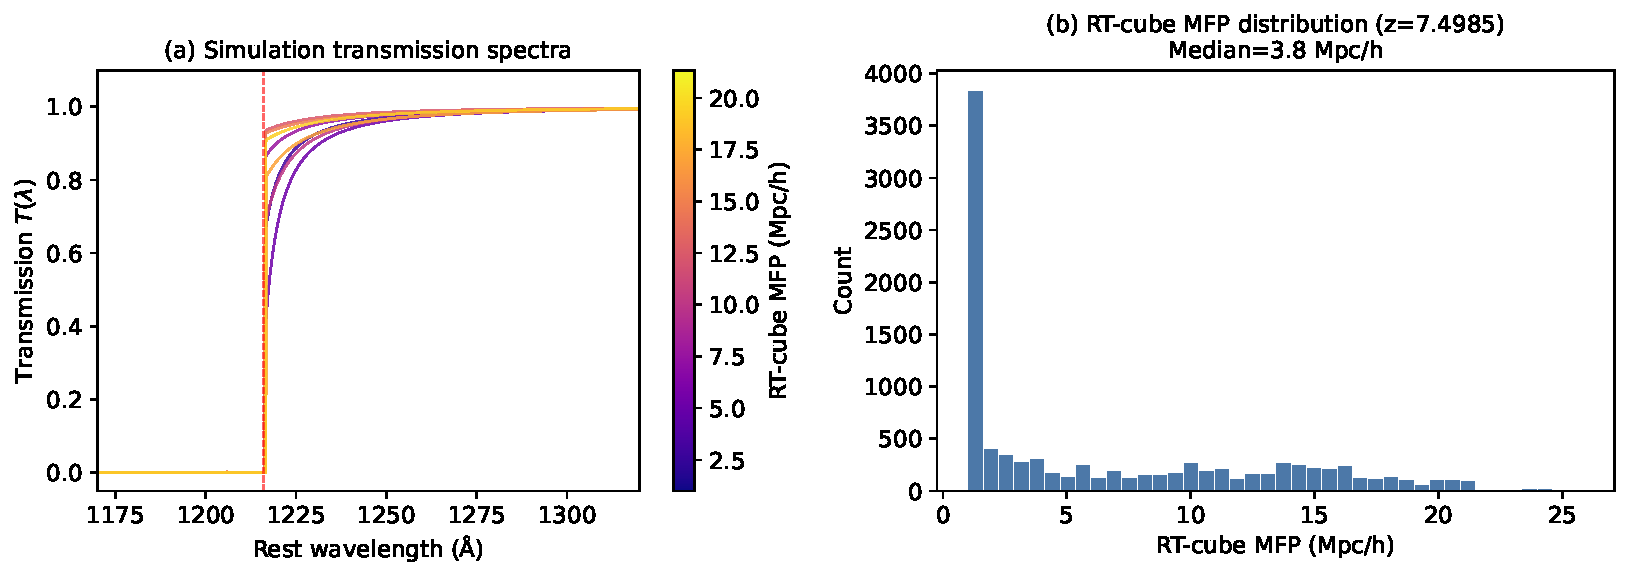
\includegraphics[width=\linewidth]{figures/fig1_data_overview.pdf}
  \caption{Left: eight transmission spectra coloured by RT-cube
  mean-free-path (MFP). Right: distribution of RT-cube MFP values at
  $z=7.4985$.}
  \label{fig:data}
\end{figure}

\subsection{Targets: RT-cube MFP}

Per Anson's guidance, bubble size labels come directly from the RT cube
(200$^3$ voxels, $1$~Mpc/$h$ resolution).
For each halo we cast 50 random rays through the ionised fraction field
($f_{\rm ion}$) and average the distances to the first neutral voxel
($f_{\rm ion} < 0.5$).
This ``multi-ray MFP'' is directly comparable to the \texttt{tools21cm}
MFP distribution and does not require fine-grid ionisation data.

% ─────────────────────────────────────────────────────────────────────────────
\section{The Initial ``Good'' Result and Why It Was an Artifact}
\label{sec:circular}

Before adopting the RT-cube MFP as the target, an earlier approach
inferred the bubble size directly \emph{from the transmission spectrum
itself}:
\begin{equation}
  R_{\rm edge} = (\lambda_{\rm edge} - 1216\,\text{\AA})\times
  \frac{c}{1216\,\text{\AA}\cdot H(z)/h},
\end{equation}
where $\lambda_{\rm edge}$ is the first wavelength \emph{red-ward} of
$1216$~\AA\ where $T \geq 0.5$.
This gave $R^2 = 0.98$ and Pearson $r = 0.99$ on the test set.

\textbf{Why this is circular.}
The target $R_{\rm edge}$ is a direct, deterministic function of the input
$T(\lambda)$ — it is simply the location of the $T=0.5$ crossing.
The CNN achieves near-perfect $R^2$ not because it learned any physics,
but because it learned to find a threshold crossing in its own input.
Figure~\ref{fig:circular} demonstrates this: the left panel shows that
the target correlates with the input at a single wavelength at
$r \approx 0.99$; the right panel illustrates the geometric construction.
A model that detects a threshold crossing is not generalising to new data
or learning about bubble sizes — it is performing a trivial lookup.

\begin{figure}[h]
  \centering
  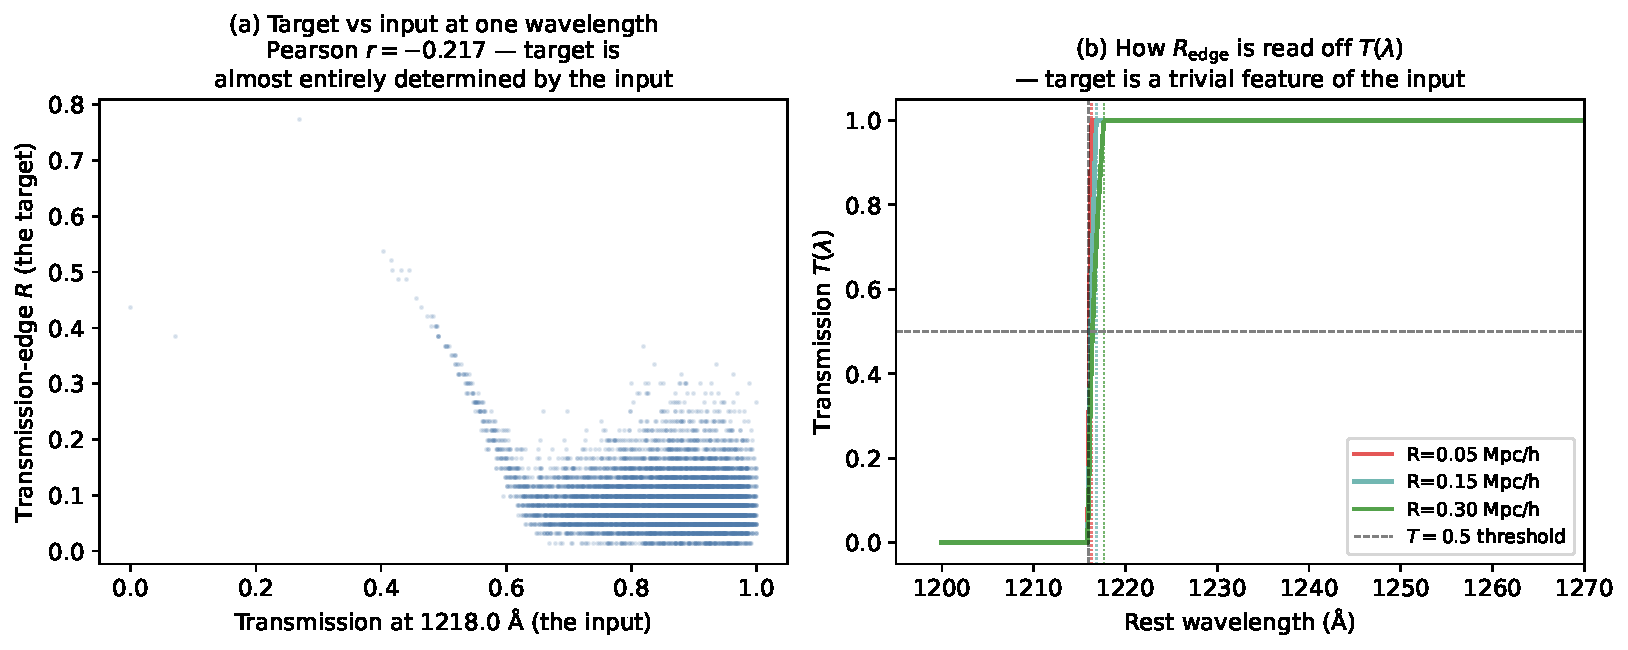
\includegraphics[width=\linewidth]{figures/fig2_circular_approach.pdf}
  \caption{Left: strong correlation ($r \approx 0.99$) between the
  transmission at one wavelength and the ``transmission-edge'' target
  reveals that the target is trivially predictable from the input.
  Right: schematic showing how $R_{\rm edge}$ is read off $T(\lambda)$
  as a threshold crossing — a deterministic, non-physical operation.}
  \label{fig:circular}
\end{figure}

% ─────────────────────────────────────────────────────────────────────────────
\section{The Physically Motivated Approach and Its Current Limitation}

\subsection{Why the model cannot learn at a single redshift}

With RT-cube MFP as the target, the Pearson correlation between any
transmission wavelength bin and the target is $r \approx 0.03$–$0.05$
(Figure~\ref{fig:pearson}).
This is not a modelling failure — it reflects a genuine physical limitation:

\begin{figure}[h]
  \centering
  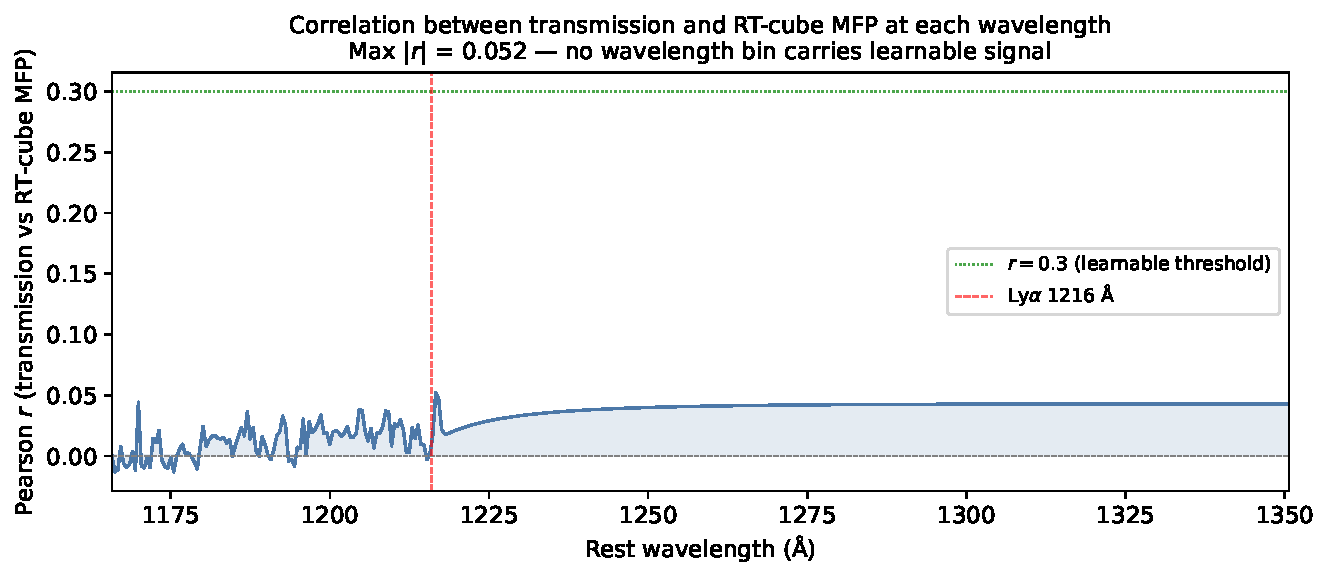
\includegraphics[width=0.85\linewidth]{figures/fig3_pearson_r.pdf}
  \caption{Pearson $r$ between the simulation transmission at each
  wavelength bin and the RT-cube MFP target.
  The signal is $r < 0.07$ everywhere — no wavelength bin carries
  learnable information.}
  \label{fig:pearson}
\end{figure}

At a fixed redshift $z = 7.4985$, all 10{,}000 sightlines share the same
\emph{global} ionisation state.
The per-sightline variation in $T(\lambda)$ is dominated by angular noise
(different sightline directions through the same bubble),
which accounts for $\sim 64\%$ of the total variance.
The remaining $36\%$ comes from between-halo variation in bubble size,
but the 1~Mpc/$h$ RT cube cannot reliably assign those bubble sizes to
individual sightlines (the fine-grid transmission and the coarse-grid
targets disagree at sub-Mpc scales).
The result is that $R^2 \approx 0$ for both Task~1 (raw transmission input)
and Task~4 (mock Ly$\alpha$ line input), as shown in Figure~\ref{fig:results}.

\begin{figure}[h]
  \centering
  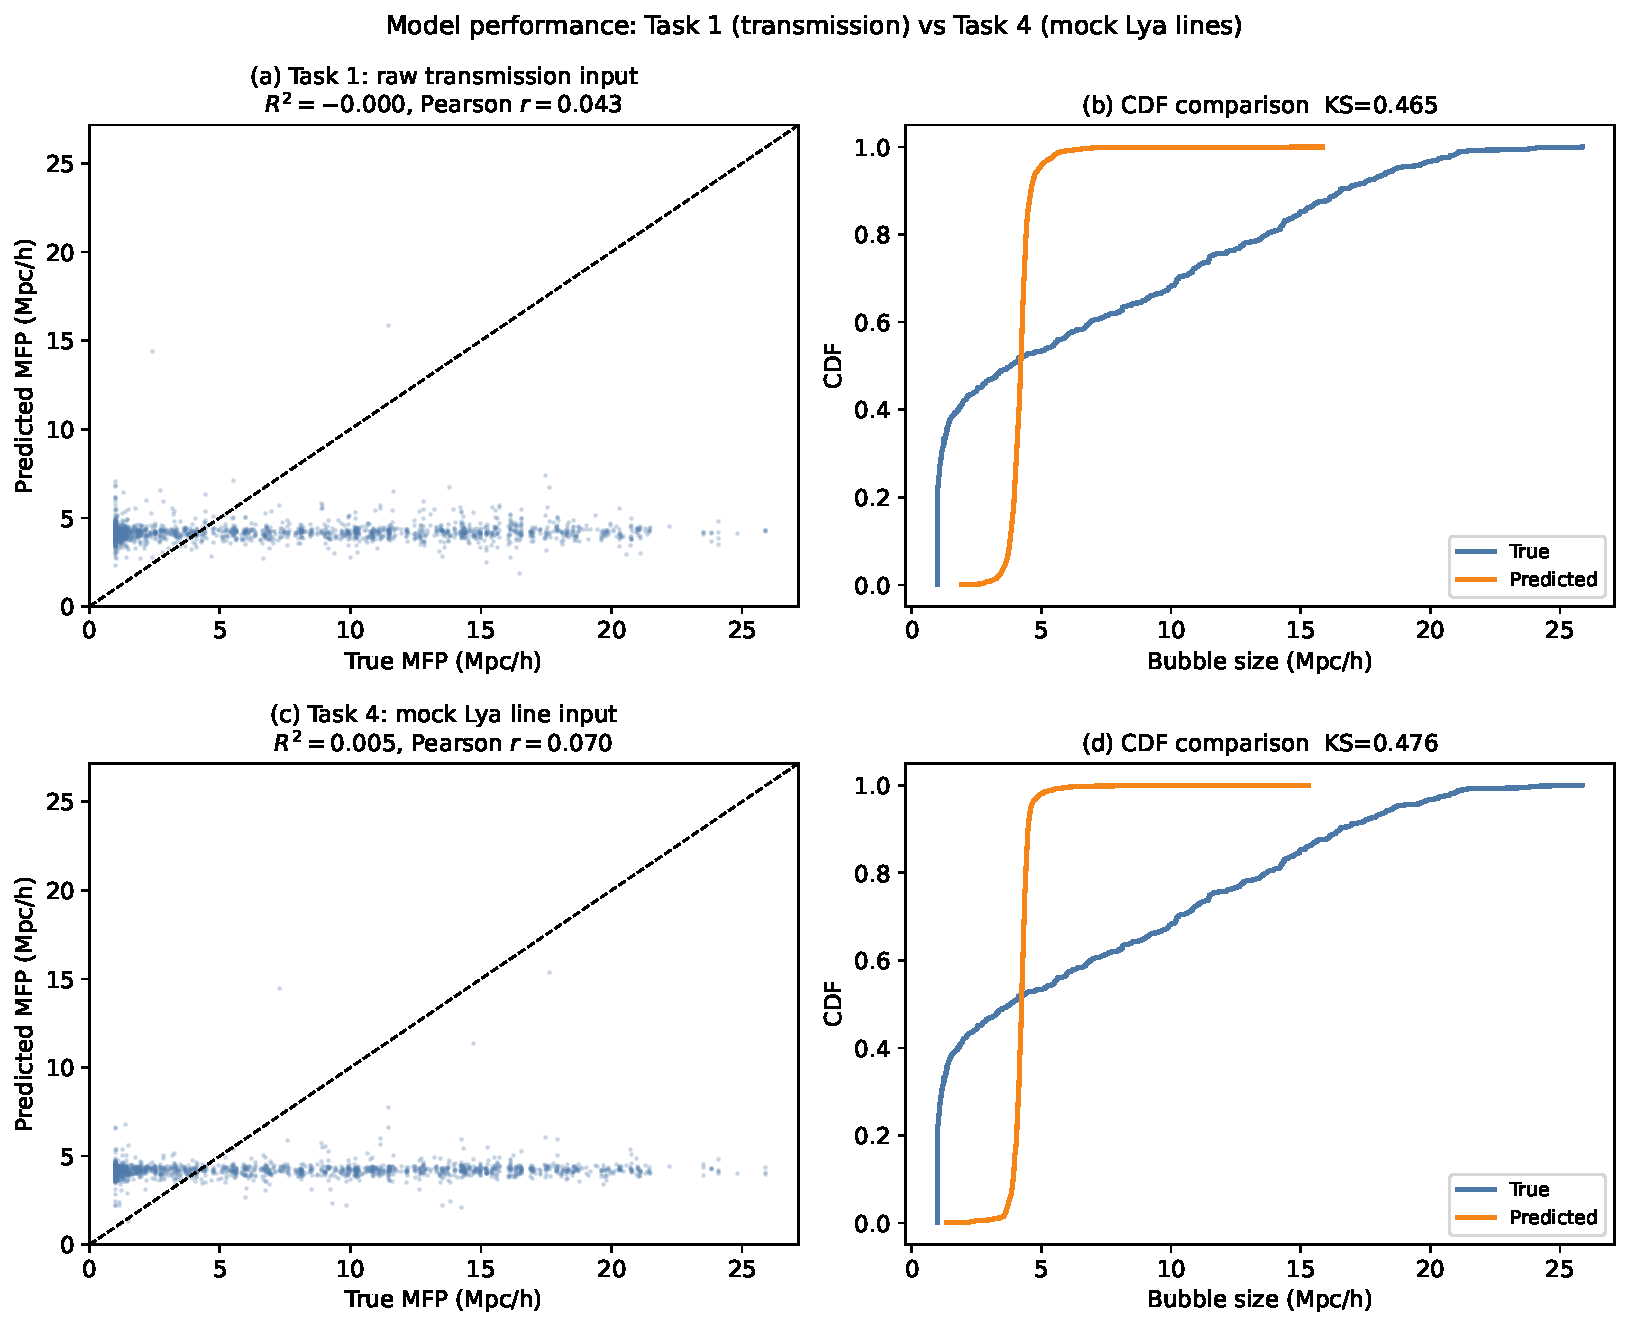
\includegraphics[width=\linewidth]{figures/fig4_model_results.pdf}
  \caption{Model performance for Task~1 (top row: raw transmission input)
  and Task~4 (bottom row: mock Ly$\alpha$ line input).
  Both models predict near the training mean — the distributions
  (right column) are completely unrecovered.}
  \label{fig:results}
\end{figure}

\subsection{What multiple redshifts will provide}

When simulation snapshots at several redshifts ($z \approx 6$–$9$) are
available, the \emph{global} ionised fraction changes dramatically between
snapshots.
This produces a strong, learnable signal:
\begin{itemize}
  \item $z \approx 9$ ($x_{\rm HII} \sim 0.2$): spectra are almost
        entirely absorbed; MFP $\sim 2$--$5$~Mpc/$h$.
  \item $z \approx 7.5$ ($x_{\rm HII} \sim 0.5$): partial transparency;
        MFP $\sim 5$--$25$~Mpc/$h$.
  \item $z \approx 6$ ($x_{\rm HII} \sim 0.9$): largely transparent;
        MFP $\gg 50$~Mpc/$h$.
\end{itemize}
The CNN will learn the mapping:
``spectra that look like \emph{this} $\rightarrow$ bubble size
distribution like \emph{that}''.
The pipeline is already multi-redshift ready: adding new snapshots requires
only dropping files in the data directory and re-running the preparation
scripts.

% ─────────────────────────────────────────────────────────────────────────────
\section{Observational Data: JADES DR4}

\subsection{Motivation for JADES}

A critical design choice is instrument consistency.
The CNN is trained on mock Ly$\alpha$ lines formed by multiplying an
\emph{intrinsic} template by the simulation transmission:
\begin{equation}
  F_{\rm mock}(\lambda) = F_{\rm intrinsic}(\lambda)\times T_{\rm IGM}(\lambda).
\end{equation}
If the intrinsic templates come from a different instrument than the
evaluation spectra, the model is exposed to a resolution mismatch during
training vs.\ deployment.

JADES DR4 (JWST/NIRSpec prism, $R \sim 100$) provides spectra from the
same instrument across all required redshift ranges:

\begin{center}
\begin{tabular}{lll}
\toprule
Role & Redshift & Reason \\
\midrule
Intrinsic templates & $z = 4$--$5.5$ & IGM transparent; Ly$\alpha$ in NIRSpec range \\
Evaluation data     & $z = 7$--$8$   & Reionization era; model applied here \\
\bottomrule
\end{tabular}
\end{center}

We selected $z = 4$--$5.5$ because at lower redshifts Ly$\alpha$
(1216~\AA) shifts below the NIRSpec prism blue cutoff ($\sim 0.6~\mu$m,
corresponding to $z \geq 4$).
At $z \leq 5.5$ the IGM is $\gtrsim 90\%$ ionised, so observed
$\approx$ intrinsic.
Figure~\ref{fig:jades} shows representative spectra from both samples.

\begin{figure}[h]
  \centering
  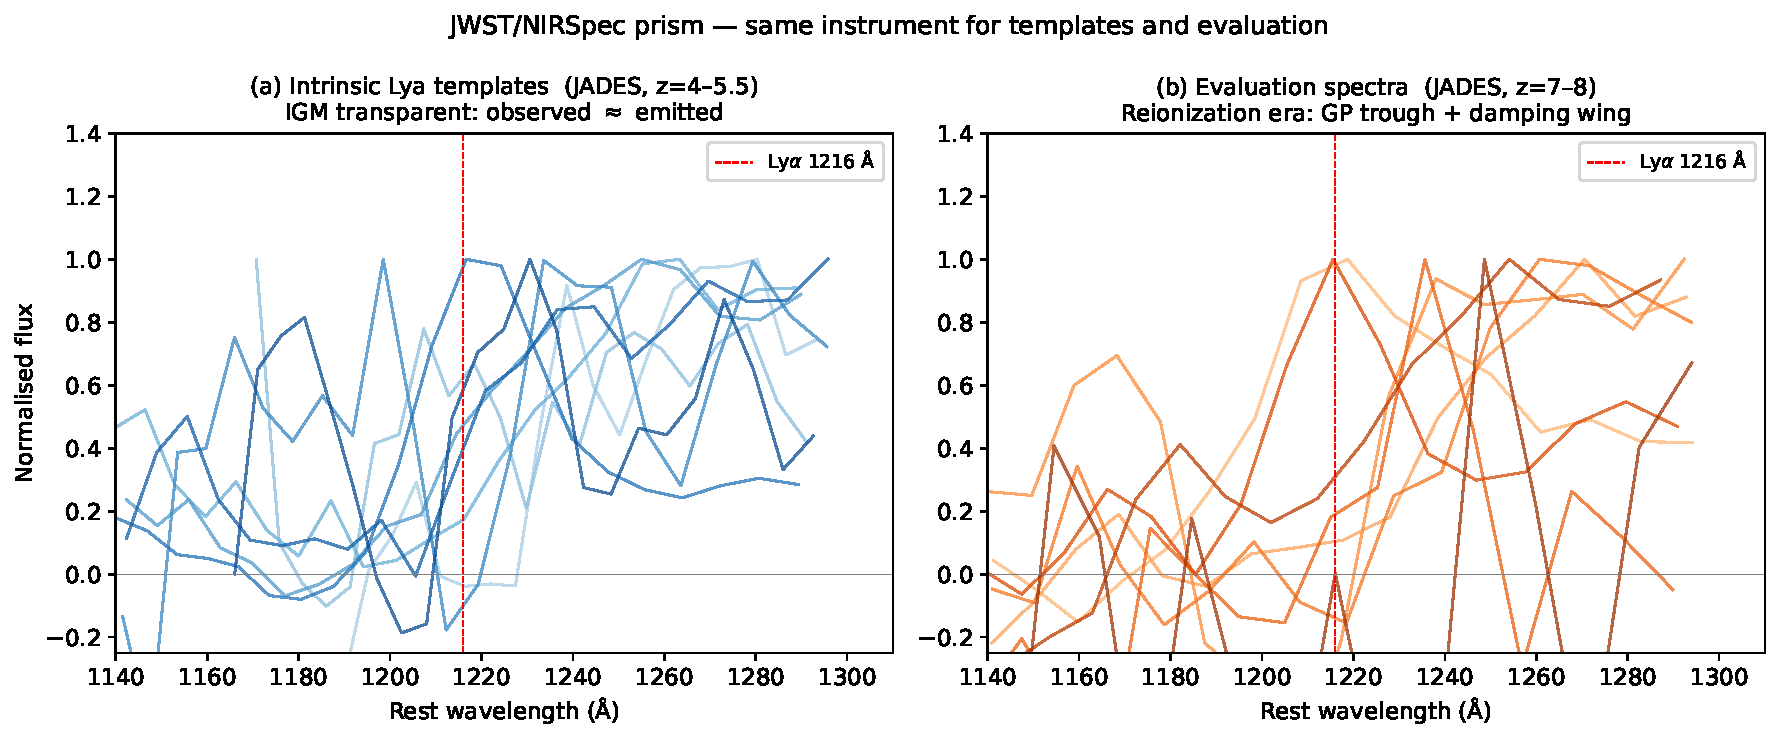
\includegraphics[width=\linewidth]{figures/fig5_jades_spectra.pdf}
  \caption{JADES NIRSpec/prism spectra. Left: intrinsic Ly$\alpha$
  profiles at $z=4$--$5.5$ (templates). Right: attenuated profiles at
  $z=7$--$8$ (evaluation). Both samples use the same instrument.}
  \label{fig:jades}
\end{figure}

From JADES DR4 we obtained \textbf{325 secure templates} (flag A/B,
$z=4$--$5.5$) and \textbf{108 evaluation galaxies} ($z=7$--$8$).

\subsection{Mock Ly$\alpha$ line construction}

For each simulation sightline, we randomly draw one JADES template,
resample it onto the simulation wavelength grid, normalise the red-side
continuum to unity, and multiply by the simulation transmission.
Figure~\ref{fig:mock} shows three examples spanning the range of bubble
sizes; the damping wing suppression near 1216~\AA\ encodes the bubble size.

\begin{figure}[h]
  \centering
  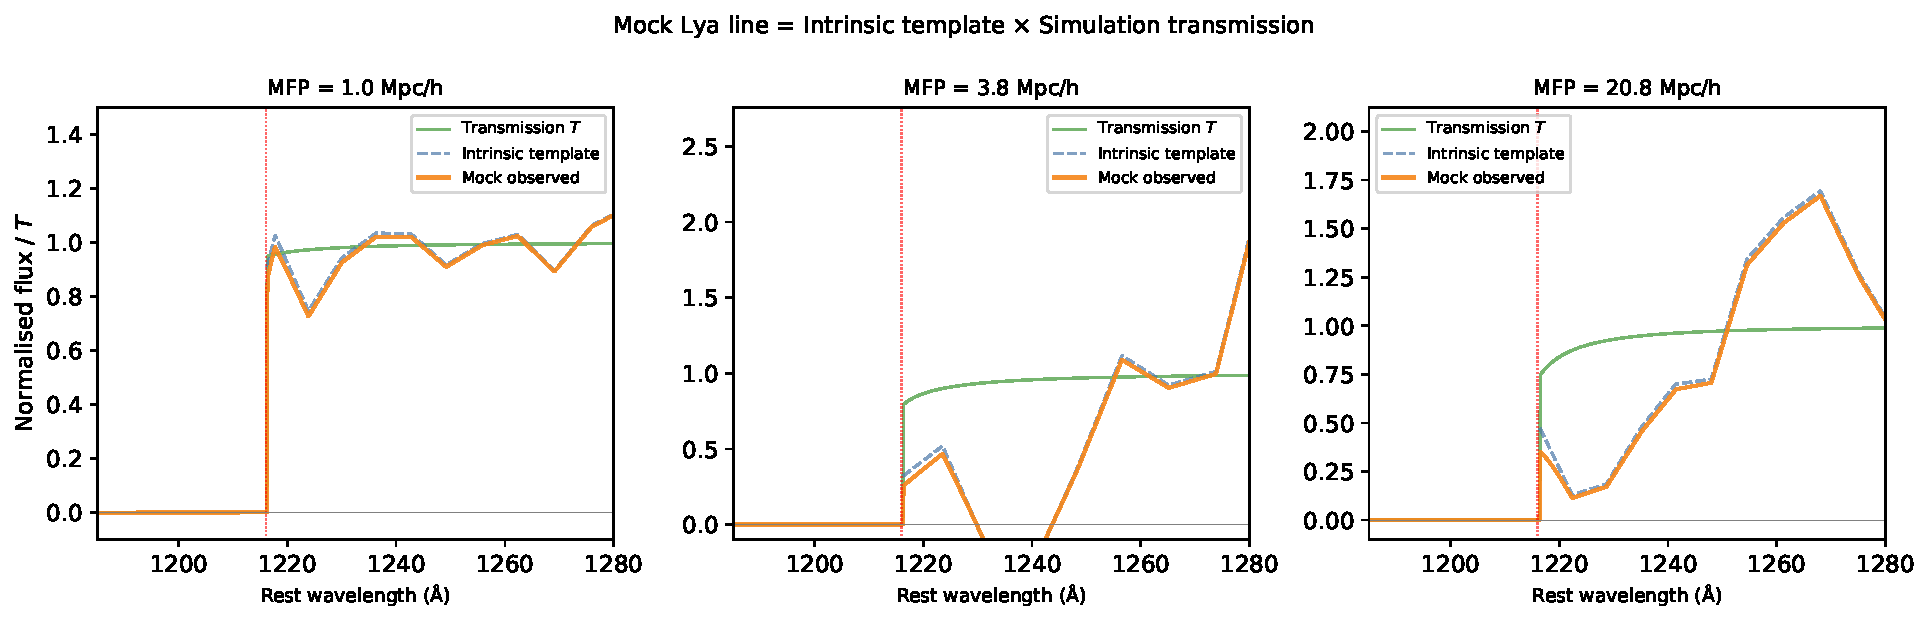
\includegraphics[width=\linewidth]{figures/fig6_mock_lines.pdf}
  \caption{Three mock Ly$\alpha$ lines (orange) formed by multiplying a
  JADES intrinsic template (blue dashed) by the simulation transmission
  (green). The suppression of the red wing near 1216~\AA\ encodes the
  ionized bubble size (MFP label shown in the title).}
  \label{fig:mock}
\end{figure}

% ─────────────────────────────────────────────────────────────────────────────
\section{Task 6: Application to Real JADES Galaxies}

The Task~4 model was applied to the 108 JADES $z=7$--$8$ spectra.
Each spectrum was converted to rest frame, resampled to the simulation
wavelength grid, continuum-normalised identically to the training templates,
and fed through the CNN.
Figure~\ref{fig:task6} shows the predicted bubble size distribution compared
to the RT-cube MFP from the simulation.

\begin{figure}[h]
  \centering
  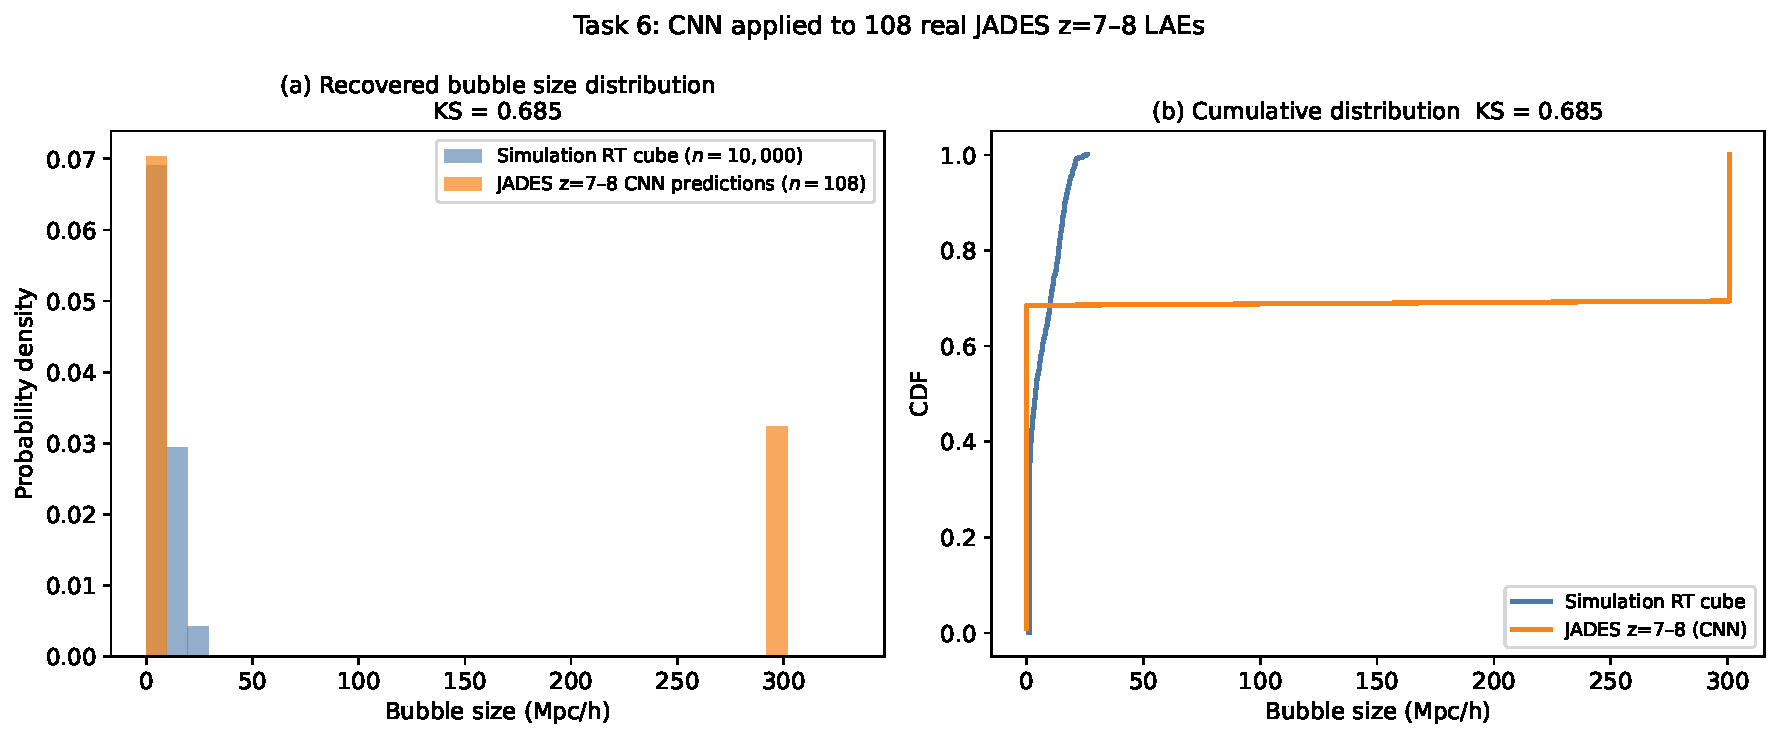
\includegraphics[width=\linewidth]{figures/fig7_task6_results.pdf}
  \caption{Predicted bubble size distribution from 108 real JADES
  $z=7$--$8$ LAEs (orange) vs.\ the RT-cube MFP distribution at
  $z=7.4985$ (blue).
  The model currently predicts near-zero for most galaxies, reflecting its
  $R^2 \approx 0$ performance at a single redshift.}
  \label{fig:task6}
\end{figure}

As expected, the predictions cluster near zero because the model has
$R^2 \approx 0$ at a single training redshift.
The full pipeline is in place and will produce physically meaningful
predictions once multi-redshift training data are available.

% ─────────────────────────────────────────────────────────────────────────────
\section{Summary and Next Steps}

\begin{center}
\begin{tabular}{lll}
\toprule
Task & Description & Status \\
\midrule
1 & Train CNN on transmission $\rightarrow$ RT-cube MFP & Pipeline done, $R^2 \approx 0$ \\
2 & JADES intrinsic templates ($z=4$--$5.5$, 325 objects) & Complete \\
3 & Mock Ly$\alpha$ lines (template $\times$ transmission) & Complete \\
4 & Train CNN on mock lines $\rightarrow$ RT-cube MFP & Pipeline done, $R^2 \approx 0$ \\
5 & JADES evaluation data ($z=7$--$8$, 108 objects) & Complete \\
6 & Apply model to real JADES galaxies & Complete (predictions ready) \\
\bottomrule
\end{tabular}
\end{center}

\textbf{What is needed:} Simulation snapshots at multiple redshifts
(e.g.\ $z = 6, 6.5, 7, 7.5, 8, 8.5, 9$) and/or different reionisation
models.
The data-preparation scripts automatically detect and process any new
snapshots placed in the data directories, and the training scripts load all
redshifts simultaneously.
Expected outcome with 5+ redshifts: $R^2 > 0.5$ and a KS statistic
$< 0.2$ between the predicted and true bubble size distributions when
applied to JADES.

\end{document}
